%%%%%%%%%%%%%%%%%%%%%%%%
%
% $Autor: Hemanth Jadiswami Prabhakaran $
% $Datum: 2025-06-25 13:26:20Z $
% $Pfad: GitHub/BA25-01-Time-Series/Presentations/WalmartSalesForecastingPresentations/slides/conclusions.tex $
% $Version: 1 $
%
% $Project: BA25-Time-Series $
%
%%%%%%%%%%%%%%%%%%%%%%%%



\Mysection{Conclusions \& Future Work}

\STANDARD{Key Contributions}
{ 
	\framesubtitle{Research \& Technical Achievements}
	
	\begin{block}{Technical Contributions}
		\begin{enumerate}
			\item \textbf{Integrated Web Platform}
			\begin{itemize}
				\item First comprehensive web-based time series forecasting system
				\item Unified training and prediction workflow
				\item Cross-platform deployment (cloud + local)
			\end{itemize}
			
			\item \textbf{Advanced Model Integration}
			\begin{itemize}
				\item Auto ARIMA + Holt-Winters implementation
				\item Automated hyperparameter optimization
				\item Performance-based model selection
			\end{itemize}
			
			\item \textbf{Interactive Business Intelligence}
			\begin{itemize}
				\item Real-time forecast visualization
				\item Color-coded trend indicators
				\item Actionable business insights
			\end{itemize}
		\end{enumerate}
	\end{block}
	
	\begin{figure}
		\centering
\begin{tikzpicture}[scale=0.8]
	% Contribution areas - increased spacing and adjusted positions
	\node[ellipse, draw, minimum width=2.5cm, minimum height=1cm, 
	fill=blue!30] (tech) at (0,3.5) {\footnotesize \textbf{Technical} \textbf{Innovation}};
	
	\node[ellipse, draw, minimum width=2.5cm, minimum height=1cm, 
	fill=cyan!20] (method) at (-4.5,1) {\footnotesize \textbf{Methodological} \textbf{Advancement}};
	
	\node[ellipse, draw, minimum width=2.5cm, minimum height=1cm, 
	fill=green!20] (business) at (3.5,1) {\footnotesize \textbf{Business}\textbf{Application}};
	
	% Central impact - moved further down
	\node[circle, draw, minimum width=2cm, fill=yellow!20] 
	(impact) at (0,-1) {\footnotesize \textbf{Accessible}\textbf{Forecasting}};
	
	% Connections
	\draw[->, thick] (tech) -- (impact);
	\draw[->, thick] (method) -- (impact);
	\draw[->, thick] (business) -- (impact);
\end{tikzpicture}
		\caption{Contribution Areas}
	\end{figure}
	
	\begin{alertblock}{Key Achievement}
		\textbf{3.58\% WMAE}: Excellent forecasting accuracy with accessible web-based deployment.
	\end{alertblock}
	
	\begin{exampleblock}{Research Questions Answered}
		\textbf{Q1}: Traditional methods (ARIMA/Holt-Winters) effectively capture retail patterns when properly optimized. 
		\textbf{Q2}: Web deployment requires careful consideration of serialization, performance, and user experience. 
		\textbf{Q3}: Interactive visualization significantly enhances forecast interpretability for business users.
	\end{exampleblock}
}

\MYNOTE{
	Summarize the key contributions and how they address the original research questions. 
	Emphasize both technical and practical achievements.
}

\STANDARD{Limitations \& Lessons Learned}
{ 
	\framesubtitle{Honest Assessment \& Insights}
	
	\begin{block}{Current Limitations}
		\begin{itemize}
			\item \textbf{Temporal Scope}
			\begin{itemize}
				\item Data: 2010-2012 (historical)
				\item May not capture recent market changes
				\item Limited long-term trend analysis
			\end{itemize}
			
			\item \textbf{Forecast Horizon}
			\begin{itemize}
				\item Fixed 4-week prediction window
				\item No dynamic horizon adjustment
				\item Limited seasonal cycle coverage
			\end{itemize}
			
			\item \textbf{Model Scope}
			\begin{itemize}
				\item ARIMA + Holt-Winters only
				\item No ensemble methods
				\item Limited external variable integration
			\end{itemize}
		\end{itemize}
	\end{block}
	
	\begin{block}{Lessons Learned}
		\begin{itemize}
			\item \textbf{Web Deployment Complexity}
			\begin{itemize}
				\item Cross-platform compatibility critical
				\item Model serialization challenges
				\item User experience paramount
			\end{itemize}
			
			\item \textbf{Business Focus Essential}
			\begin{itemize}
				\item Technical accuracy $\neq$ business value
				\item Interpretation matters more than precision
				\item Accessibility drives adoption
			\end{itemize}
			
			\item \textbf{Iterative Development}
			\begin{itemize}
				\item Continuous testing essential
				\item User feedback invaluable
				\item Performance optimization ongoing
			\end{itemize}
		\end{itemize}
	\end{block}
	
	\begin{exampleblock}{Key Insight}
		The most sophisticated algorithm is useless if it's not accessible to the people who need to make decisions based on its output.
	\end{exampleblock}
}

\MYNOTE{
	Be honest about limitations while emphasizing the valuable lessons learned. 
	This shows critical thinking and sets up future work opportunities.
}

\STANDARD{Future Work \& Enhancements}
{ 
	\framesubtitle{Roadmap for Continued Development}
	
	\begin{figure}
		\centering
			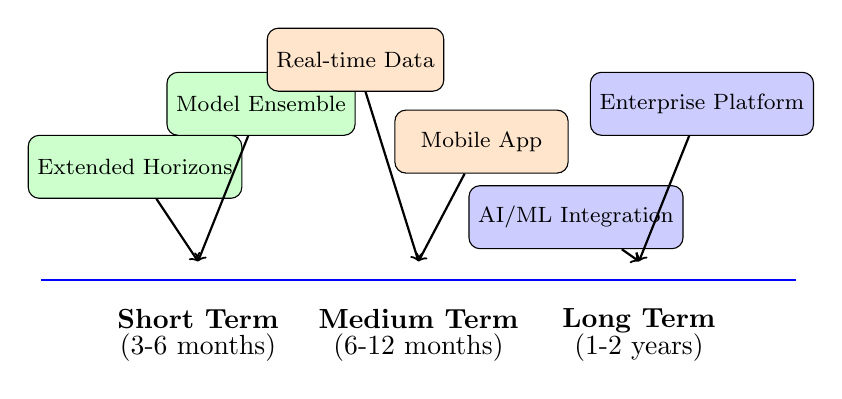
\begin{tikzpicture}[scale=0.8]
	% Timeline - moved up
	\draw[thick, blue] (0,2.5) -- (12,2.5);
	
	% Time periods - moved up
	\node[below] at (2.5,2.2) {\textbf{Short Term}};
	\node[below] at (2.5,1.8) {(3-6 months)};
	\node[below] at (6,2.2) {\textbf{Medium Term}};
	\node[below] at (6,1.8) {(6-12 months)};
	\node[below] at (9.5,2.2) {\textbf{Long Term}};
	\node[below] at (9.5,1.8) {(1-2 years)};
	
	% Short term enhancements - moved up
	\node[rectangle, draw, rounded corners, minimum width=2.2cm, minimum height=0.8cm, 
	align=center, fill=green!20] (short1) at (1.5,4.3) {\footnotesize Extended Horizons};
	\node[rectangle, draw, rounded corners, minimum width=2.2cm, minimum height=0.8cm, 
	align=center, fill=green!20] (short2) at (3.5,5.3) {\footnotesize Model Ensemble};
	
	% Medium term enhancements - moved up
	\node[rectangle, draw, rounded corners, minimum width=2.2cm, minimum height=0.8cm, 
	align=center, fill=orange!20] (med1) at (5,6) {\footnotesize Real-time Data};
	\node[rectangle, draw, rounded corners, minimum width=2.2cm, minimum height=0.8cm, 
	align=center, fill=orange!20] (med2) at (7,4.7) {\footnotesize Mobile App};
	
	% Long term enhancements - moved up
	\node[rectangle, draw, rounded corners, minimum width=2.2cm, minimum height=0.8cm, 
	align=center, fill=blue!20] (long1) at (8.5,3.5) {\footnotesize AI/ML Integration};
	\node[rectangle, draw, rounded corners, minimum width=2.2cm, minimum height=0.8cm, 
	align=center, fill=blue!20] (long2) at (10.5,5.3) {\footnotesize Enterprise Platform};
	
	% Arrows to timeline - adjusted connection points
	\draw[->, thick] (short1) -- (2.5,2.8);
	\draw[->, thick] (short2) -- (2.5,2.8);
	\draw[->, thick] (med1) -- (6,2.8);
	\draw[->, thick] (med2) -- (6,2.8);
	\draw[->, thick] (long1) -- (9.5,2.8);
	\draw[->, thick] (long2) -- (9.5,2.8);
\end{tikzpicture}
		\caption{Development Roadmap}
	\end{figure}
	
	\begin{block}{Short Term (3-6 months)}
		\begin{itemize}
			\item \textbf{Extended Horizons}: 8-12 week forecasts
			\item \textbf{Ensemble Methods}: Model combination
			\item \textbf{Performance Tuning}: Speed optimization
			\item \textbf{Additional Models}: Prophet, LSTM
		\end{itemize}
	\end{block}
	
	\begin{block}{Medium Term (6-12 months)}
		\begin{itemize}
			\item \textbf{Real-time Data}: API integration
			\item \textbf{Mobile Application}: iOS/Android apps
			\item \textbf{Advanced Analytics}: Confidence intervals
			\item \textbf{User Management}: Multi-user support
		\end{itemize}
	\end{block}
	
	\begin{block}{Long Term (1-2 years)}
		\begin{itemize}
			\item \textbf{AI Integration}: AutoML capabilities
			\item \textbf{Enterprise Platform}: Commercial deployment
			\item \textbf{Industry Expansion}: Beyond retail
			\item \textbf{Research Platform}: Academic collaboration
		\end{itemize}
	\end{block}
}

\MYNOTE{
	Present a realistic and exciting vision for future development. This shows 
	forward thinking and potential for continued research and application.
}

\STANDARD{Final Thoughts}
{ 
	\framesubtitle{Impact \& Significance}
	
	\begin{block}{Project Impact}
		\begin{itemize}
			\item \textbf{Academic Contribution}
			\begin{itemize}
				\item Demonstrates practical time series deployment
				\item Bridges theory-practice gap
				\item Provides open-source foundation
			\end{itemize}
			
			\item \textbf{Business Value}
			\begin{itemize}
				\item Accessible forecasting for SMEs
				\item Rapid prototype development
				\item Cost-effective solution
			\end{itemize}
			
			\item \textbf{Technical Innovation}
			\begin{itemize}
				\item Web-based ML deployment patterns
				\item Cross-platform compatibility solutions
				\item Interactive visualization best practices
			\end{itemize}
		\end{itemize}
	\end{block}
	
	\begin{figure}[H]
		\centering
		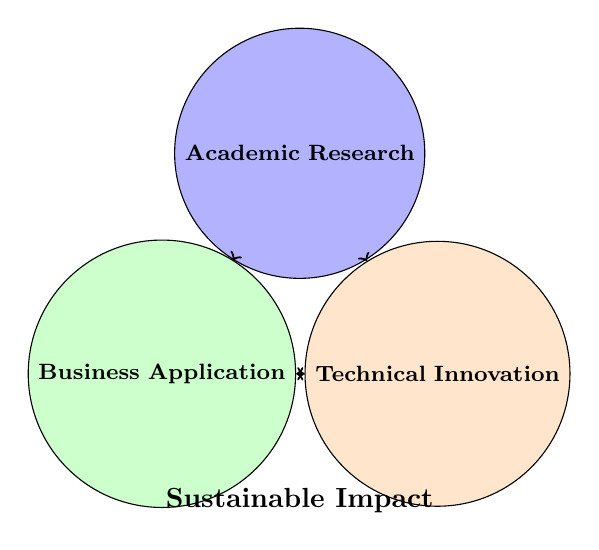
\begin{tikzpicture}[scale=0.7]
	% Impact circles - increased spacing to prevent overlap
	\node[circle, draw, minimum width=1.8cm, fill=blue!30, align=center] 
	(academic) at (0,4) {\footnotesize \textbf{Academic}  \textbf{Research}};
	
	\node[circle, draw, minimum width=1.8cm, fill=green!20, align=center] 
	(business) at (-2.5,0) {\footnotesize \textbf{Business}  \textbf{Application}};
	
	\node[circle, draw, minimum width=1.8cm, fill=orange!20, align=center] 
	(tech) at (2.5,0) {\footnotesize \textbf{Technical}  \textbf{Innovation}};
	
	% Connections - bidirectional arrows between business and tech
	\draw[->, thick] (academic) -- (business);
	\draw[->, thick] (academic) -- (tech);
	\draw[<->, thick] (business) -- (tech);
	
	% Central impact
	\node[font=\bf] at (0,-2.3) {Sustainable Impact};
\end{tikzpicture}
		\caption{Multi-dimensional Impact}
	\end{figure}
	
	\begin{alertblock}{Success Metrics}
		\begin{itemize}
			\item \checkmark \textbf{Excellent accuracy}: 3.58\% WMAE
			\item \checkmark \textbf{User-friendly}: Web-based access
			\item \checkmark \textbf{Scalable}: Cloud deployment
			\item \checkmark \textbf{Practical}: Business-focused
		\end{itemize}
	\end{alertblock}
	
	\begin{exampleblock}{Closing Reflection}
		This project demonstrates that sophisticated time series forecasting can be made accessible 
		without sacrificing statistical rigor, opening new possibilities for data-driven 
		decision making in retail and beyond.
	\end{exampleblock}
}